\def \coursename  {CM3070 CS Final Project}
\def \assigntment {Preliminary Report}
\author {Hayato Ishida}

\documentclass[11pt, natbib=false]{article}

\usepackage{url}
\usepackage{hyperref}
\usepackage{fancyhdr}
\usepackage{multicol}
\usepackage{listings}


\setlength{\columnsep}{1cm}
\usepackage[backend=bibtex,
            sorting=none,
            citestyle=numeric,
            style=ACM-Reference-Format]{biblatex}
\addbibresource{refrence.bib}
\usepackage{geometry}
\geometry{margin=2cm}

\usepackage{graphicx}
\usepackage{subcaption}

\setlength\parindent{2em}
\setlength\parskip{0em}
\renewcommand{\baselinestretch}{1.5}
\linespread{1.3}

% \pagestyle{fancyplain}
% \chead{\assigntment}
\date{\today}
\title{Final Project Draft Report}

\begin{document}

\maketitle

\begin{multicols}{2}
\section{Introduction}
These days, many human-to-human interactions are taking place on online platforms, mainly in social media.
Many comments are being exchanged on a wide range of topics within social media, but those are not necessary all using appropriate languages ~\cite{hada2021ruddit}.
Some of the contents may include offensive or hateful language, and exposure to those contents can affect users’ mental health well-being ~\cite{hada2021ruddit}.

In recent years, there has been increasing attention towards violence on social media platforms in the general public.
In Japan, young TV star suicide was caused by offensive and violent comments targeting a specific person ~\cite{HanaK}.
Following that incident, there was lots of focus on online insulting with offensive or abusive language. The Japanese government considers stricter law enforcement against those insulting on social media platforms ~\cite{JpGov}.
COVID-19 pandemic was declared by WHO in March of 2020 ~\cite{whoCovid}.
Since then, many countries have placed various major restrictions to fight this disease, including social distancing and lockdowns. Social media plays a vital role in connecting people during that time. Although it brought lots of benefits to our society, there is also a dark side ~\cite{liu2021covid}.
A study ~\cite{babvey2021using} shows an increase in abusive content or comments on Twitter and Reddit in several countries, specifically countries with strong restrictions.

A system for detecting offensive, abusive and hateful content attracting more interest from social media providers and regulators ~\cite{vidgen2019challenges}.
Specifically, there is growing concern about the effect of those content on the mental health of younger generations ~\cite{babvey2021using}.
At the same time, due to ambiguous and diverse definitions of offensive content, it is a challenging topic for the research field of NLP and machine learning ~\cite{vidgen2019challenges}.

This project attempts to develop a machine learning model that has overcome several challenges: classifying diverse offensive content and short text.
The model should return a degree of offensiveness in numerical value instead of a specific class.
This model can be a solution to overcome the ambiguity and diverseness of offensive content.
Also, it will use genetic algorithms to automate the optimization process of neural network architecture ~\cite{andersen2021evolving}. 
Genetic algorithm is a searching algorithm inspired by the theory of evolution developed by Charles Darwin in 1859.
With this algorithm, the optimized neural network possibly developed automatically.

This project is based on the final project template of Machine Learning and Neural Network: deep learning on a public dataset.
In addition, the project is partially inspired by the Artificial Intelligence project template: automated design using evolutionary computation.
Also, include knowledge and programming techniaues of Natural Language Processing. 

\section{Literatures Review}
Since this is a well-established topic of research in Machine Learning and Natural Language Processing, several studies are related to offensive language detection. 

Malmasi Shervin and Zampieri Marcos ~\cite{malmasi2017detecting} demonstrate a text classification model to classify hate speeches in social media. This study developed a supervised classification model using a publicly published dataset of tweets from Twitter.
The study used surface n-gram and word skip grams features, which have proven to work well with this task. The study uses support vector machines with LIBLINEAR package for a classifier model because of their high performance with similar word classification.
The package, However, the study also demonstrates some problems with hate speech classification. First of all, each tweet of the dataset was labeled by individuals into three different classes: Hate, offensive, and ok.
There is some ambiguity of definitions between ‘hate’ and ‘offensive.’ In the usual sense, different individuals would get different impressions from the same content.
For example, with the same violent tweet, some might think it is ‘offensive,’ but others might think it is instead ‘hate.’
The result of this study exactly shows the ambiguity of those class definitions. The classification model successfully distinguishes the ‘ok’ tweet from the other two. However, the model performance was not good enough to distinguish between ‘hate’ and ‘offensive’; also, some ‘hate’ or ‘offensive’ tweets are classified as ‘ok.’
This result demonstrates that there is an overlap of definition between those three classes because of ambiguity of language.
The study shows that this is not practical to use specific classes to detect any hate or offensive content on social media platforms.
It is necessary to overcome that ambiguity of language to build a practical and effective text classification model. 

The study by Rishav Hada et al. ~\cite{hada2021ruddit} also points out those ambiguous definitions of different types of offensive languages.
This study is similar to Malmasi Shervin and Zampieri Marcos ~\cite{malmasi2017detecting} but approaches the problem differently.
Classifying offensive language is quite complicated because there are many possible classes such as racist, sexist, hate speech, offensive, hateful, etc. In the real world, those classes can be ambiguous and overlap.
In addition to those ambiguities, swear words are another problem that offensive text classification must consider.
It is easy to classify them as offensive, but text with swear words does not necessarily mean offensive.
For instance, ‘Hell yes, and ‘sure as hell love it’ are not offensive.
Those comments use swear words to express their feelings.
However, those words are surely inappropriate languages.
This study overcomes the ambiguity of offensive words by giving each data the best-worst scaling between -1 and 1, where -1 is maximally supportive, and 1 is maximally offensive.
This approach allows classification tasks to be less ambiguous.
Although each person will take an offensive text differently, it will not cause different classes to overlap.
The study consider three different computational models: Bidirectional LSTM ~\cite{pennington2014glove}, BERT ~\cite{devlin2018bert}, and HateBERT ~\cite{caselli2020hatebert}.
As a result, HateBERT performs the best, and considering its publication date, it is a good result. 

The previous two studies give a clear insight into distinguishing between different types of offensive languages on social media or the internet platforms.
The following study shows the negative effects of offensive words on young people.

The paper by Shi Xiaoqin, Yu Chao, and Wu Dongmei ~\cite{shi2021influence} study how those violent languages on the Internet affect young students' mental health.
Most young students are users of the Internet, and it is hard to find a young student who does not have a social media account.
The study focuses on young students because they are most vulnerable to that language violence on the Internet.
Young people are in the middle of physical and mental development, and the study concern the negative effect of language violence during that development.
A survey to each student collects data. The study shows that there are many different negative effects on young students’ mental health, and an attempt of psychological intervention to improve their mental health did not bring significant positive results.
All of those negative psychological effects lead to various problems for young students.
It can cause problems in daily life activities such as sleeping, eating, and interpersonal relationships. It can also cause mental health-related problems, including feelings, emotions, and consciousness.
Those problems can lead to other problems for young students, as well. To improve those psychological problems, the improvement of online platforms is necessary.
Unfortunately, some online platforms ignore those language violences and gain some attention to maintain or increase traffic and for another benefit.
This leads to more violence. Adults are likely to have the capability to avoid those contents or deal with those contents.
However, young people are not capable of dealing with those content. Therefore, some sort of protection is necessary for them.
Although the data sample of this study is small, it still shows the significance of those adverse effects caused by language violence on the Internet.
An efficient violent language detecting system is the possible solution for this issue. 

The study by Rishav Hada et al. ~\cite{hada2021ruddit} proposed some efficient text classification methods to detect offensive language.
The study by Andersen Hayden et al. ~\cite{andersen2021evolving} shows the possibility of using a genetic algorithm to construct an efficient text classification model automatically.
Genetic algorithm is a bio-inspired searching algorithm that can bring solutions beyond our imagination ~\cite{lehman2020surprising}.
One of the main issues in developing text classification is the requirement of knowledge.
Convolutional Neural Network is known for its high performance in text classification tasks. To develop text classification with a Convolutional Neural Network, deep knowledge of natural language processing and deep learning, a combination of machine learning and neural networks, is necessary.
Also, constructing this type of text classification model is not easy to do in general. Considering those challenges, this study attempt to automate the construction process by genetic algorithm.
Although it is still an initial stage of this area of research, this study shows various possibilities of applying genetic algorithms to text classification tasks.
The study presents two similar methods but different slitty approaches. Genetic algorithm representation is essential, and it presents two different ways: vector and tree-like graphs.
The vector representation is relatively simple and easier to work with.
The downside of this study is computational cost.
It requires quite a lot of computation cost to run a genetic algorithm.
However, it can be controlled flexibly by adjusting population size and number of generations.
As a result, the study developed well perform text classification model.
The result of the study provides evidence that the genetic algorithm can be used for machine learning model development, and it is pretty compelling. 

A text on social media platforms or any other online platform can be pretty short. For instance, content on Twitter is relatively short. The platform has a word limit of 280 characters [15].
Classifying short text is not an easy task.
The study by Wang Haitao ~\cite{wang2021short} presents a method to tackle this difficult task.
First of all, in-text classification task, the short text is harder to deal with for some reason. This is simply because of its lack of necessary information for text classification.
The study uses Convolutional Neural Network because of its promised performance in a text classification task. It goes through four steps to do short text classification.
First, it uses Jaro–Winkler similarity to detect any spelling error on text. Spell miss can lead to entirely different output in the short text.
Secondly, it finds related words to extend the semantics of short text. Finally, conceptualize short text and then extract short text features.
As a result, the study successfully improved the performance of short text classification.
Combining this technique with a traditional text classification method in a real-world application can be pretty challenging.
However, at the same time, it is a necessary technique to apply text classification to various content on online platforms. 

Those studies consider various methods to construct well perform text classification model.
Therefore, the results of those studies are a beneficial source to consider the methodology to this project of offensive language rating. 



\section{Design}
\subsection{Overview}
The main objective of this project is to develop an offensive language detection model using Machine Learning and Neural Network knowledge.
The project also involves some knowledge from Natural Language Processing and Artificial Intelligence. The model aims to detect various offensive languages on online platforms, including social media platforms and other platforms that allow users to leave a comment.
The project only considers one language, which is English.
Reasons for this will be explained in a later section.
This area of research is one of the main focuses in the Natural Language Processing research community, mainly because of increasing online platforms.
Offensive language detection is the necessary technology to keep online platforms healthy in many ways ~\cite{vidgen2019challenges}. A conventional text detecting model classifies a text into a specific class.
For instance, particularly to this project’s topic, classes can be ‘hate,’ ‘violence,’ ‘offensive.’ ‘ok,’ etc. The language is often very ambiguous, and it is always a challenge that natural language processing face.
Of course, this ambiguity applies to offensive language, as well. Categorization is a crucial part of modeling the Machine Learning model.
Categorization is complex in offensive language because of its variety ~\cite{vidgen2019challenges}.
There are many possible ways to categorize them. The general approach would be to categorize them into simple classes such as ‘hate,’ ‘offensive,’ ‘ok,’ etc. However, different researchers use a different level of abstraction and can be pretty unclear ~\cite{vidgen2019challenges}.
There is research ~\cite{malmasi2017detecting} that shows results that demonstrate how abstracted class categorization is complex for the Machine Learning model, particularly for this area of research.
To overcome this challenge, a study by a group of researchers from the Alan Turing Institute ~\cite{vidgen2019challenges} proposed a different way of categorizing offensive language.
Also, the study by Rishav Hada ~\cite{hada2021ruddit} proposes rating each text with a degree of offensiveness which is a pretty different approach compared to the conventional Machine Learning model.
This project uses a second approach to construct a Machine Learning model.
When constructing a Machine Learning model, tuning parameters can be quite challenging.
Also, it will require much time and human resources, in this case, myself.
This project will use a genetic algorithm to automatically tune parameters for building Machine Learning models and construct Neural Networks.
A genetic algorithm can take a long time to run, but it can run without the presence of a human.
Also, this will be interesting to see what level of creativity can genetic algorithm provide to construct a deep Machine Learning model.
There is one more thing that the project needs to consider, which is short text classification.
Since short text lacks the necessary contextual information to train the Machine Learning model ~\cite{wang2021short}.
Online platforms and social network platforms are full of short text.
This part might become necessary to this project, but it is not the main focus. 

\subsection{Templeate of this project}
The main template of this project is Deep Learning on a public dataset from CM3015 Machine Learning and Neural Networks. Also, this project overlaps with another template: Automated design using evolutionary computation from CM3020 Artificial Intelligence. In addition to these templates, some knowledge from CM3070 Natural Language Processing will contribute to this project. 

\subsection{Domain and users}
The primary users for this project are young adult internet users and online platform providers such as social network platforms.
Most young adults are users of various online platforms, and not all platforms have proper regulations and technologies against offensive languages.
The various negative effects of offensive language from the online platform are concerning ~\cite{babvey2021using}~\cite{shi2021influence}.
Also, it became essential for online service providers to have a robust system to detect offensive languages to provide safe platforms ~\cite{vidgen2019challenges}.
This project can also contribute to various psychological research related to negative psychological effects on mental health, such as the study about young students’ mental health ~\cite{shi2021influence}.

Inappropriate language detecting application is the primary domain for this project.
Protecting people’s mental health from offensive language is also a part of the domain.
This technology area is still considered a challenging area of research, and not all online platform providers can adopt those into their service.
Also, big technology companies have already placed systems to reduce the amount of offensive language within service, but there is still room for improvement.
Nevertheless, this area of research can contribute to protecting people’s mental health against unhealthy online behaviors. 

Today, the Internet is available in most places in the World and even in space.
Therefore, hundreds of different languages are used on various online platforms.
This project focuses on English because it is one of the most common languages in the World.
However, it is possible to apply this project to other languages in further works to reach a broader range of users.
Offensives language detecting systems related works perform well.
However, it sometimes detects regular comments as offensive or offensive language gets around the system.
Also, there is a challenge with an unclear categorization of offensive language and overall ambiguity of offensive language.
Overcoming those challenges can provide a better detecting system.
Furthermore, it is automating tuning process can implementation process more accessible for those online platform providers and make this project adaptable to different topics of text classification. 

\subsection{Overall Structure}
This project will follow the basic steps of deep learning model development.
The first steps will be data installation and pre-processing.
This process involves installing all necessary datasets into a machine’s local environment.
Then pre-process these datasets as necessary, including formatting, data cleaning, and split into train, test, validation datasets.
In the second step, the project will carry out some data analysis on the dataset to better understand the dataset, which includes some fundamental Natural Language analysis.
The actual deep learning model construction will take place next.
The base model will be from the research ~\cite{hada2021ruddit}, which shows the most effective and relates to this project the most.
However, the project will consider different choices from other related works.
As part of model construction, a genetic algorithm will search for the best-performing parameter combination. 

In this project, there are various technologies involved.
The most important technologies are the deep learning model, which consists of various knowledge, including Machine Learning and Neural networks.
Also, knowledge of Natural Language is vital for this project to succeed.
In addition, genetic algorithms play an essential role in automating some parts of the project and provide some creativity.

Another important aspect of this project is evaluation.
The result of model performance will be analyzed with Pearson correlation, MSE, and error analysis as the study by Rishav Hada ~\cite{hada2021ruddit} analyzes their data.
To evaluate this project, the result will be compared with other related works.
Since rating offensive language with numerical values is somewhat subjective, testing will require a third party to see the result.
However, this type of test can be carried out with some users. 

\subsection{Project Plan}
Project planning is a crucial criterion for a successful project. Detail plan for this project is gathered on one Gantt chart below ((a) Gantt Chart on Figures section).
The plan is set weekly, and the week count is the same as the UoL module scheduling system.
It starts from Week 9, the following week of peer graded assignment submission for project design.
There are some extra weeks of work plan in important parts of this project.
Last 5 weeks of implementation are dedicate towards evaluation, testing and implementation of a model.
Testing and evaluation are critical part of the project, and project can be improved based on result of those.
For a write up task, additional draft is included to make sure its quality is high at the final submission.
Also, for that purpose, the last 2 weeks of the project is dedicate for write up only.
Also, those extra weeks are for cases where thighs did not go as planned.
Putting some insurance in planning ensures that the project will be completed on time. \\
\\
\\
\\

\section{Implemementation}
\subsection{Overviwe}
The main objective of this project is to develop an offensive language detection deep learning model with the genetic algorithm.
The model aims to classify offensive languages between the scale of -1 (not offensive) and 1 (very offensive).
In addition, the genetic algorithm will be used to improve the model automatically.
By the date of this report, implementations are focused on developing the base model.

\subsection{Dataset}
Dataset for this project was obtained from Ruddit research paper ~\cite{hada2021ruddit}.
The dataset is available on the GitHub page of the paper.
However, the dataset only contains the id of each comment.
Therefore, each comment has to retrieve using Reddit API.
This process only requires a couple of lines of Python script ((d) on the figures section).

This Python code iterates through each row of the original dataset and converts comment id into actual comment using Reddit API.
Some comments no longer exist on Reddit, which are removed from the dataset.


\subsection{Model}
The main components of the initial prototype of the model are convolutional layers and a pre-trained GloVe word vector. From the performance of the prototype, convolutional layers show some promise performance.
Models from the Ruddit research paper ~\cite{hada2021ruddit} were considered in the first implementation. Although the Ruddit paper uses the PyTorch library, this project uses the TensorFlow library.
Bert and HateBert models perform well on the Ruddit research; however, there is a downside.
The size of both models are enormous, and there is no access to the hardware that can handle those model with a decent time. For that reason, a different mode was considered, the BiLSTM model.
This model is one of the models that the Reddit paper used. There are two different implementations at this date.
Both with the same model but different tokenizers.
One with BERT tokenizer ~\cite{devlin2018bert} and another with HateBERT ~\cite{caselli2020hatebert} tokenizer.
These two implementations have somewhat experimental elements.
Models are implemented based on how it is implemented on Reddit but slightly different.
The model is a combination of Convolutional layers and BiLSTM layers.
This combination had a better result than a model with just BiLSTM layers.
Please refer to the (b) on the figures section.


\section{Evalutation}
Evaluation is carried out with Mean Square Error, which is also used for the loss function on model training.
Also, accuracy is calculated in part of the evaluation.
Since the model is trained to classify each comment with a value, it classifies the result as accurate if the absolute difference between actual and predicted values is within a specific range. Finally, detailed results are shown in the table. Please refer to the (c) Result of model prediction on the figure section velow.

Overall, MSE is not low as the model from Reddit.
Accuracy is pretty high with 0.3 differences.
However, there is plenty of room to improve the model, and the genetic algorithm should be a helpful tool. By implementations so far, the base model is constructed but still needs improvement.
Also, more efficient evaluations, including unit testing, are necessary for further development.


\section{Conclusion}
The usage of offensive and inappropriate language is a significant problem that everyone needs to consider on the modern internet, especially where people can use their own words.
The development of this project up to this date suggests that the deep learning model can be developed and used to evaluate the offensiveness of English sentences.
However, it is a challenging task, and different considerations need to be taken.

There is still much room for improvement and development required in this project.
Also, different approaches need to take place, including developing own tokenizers and developing the model using the genetic algorithms.
Then, more experimental elements can take this project with more successful results.

\newpage
\printbibliography
\end{multicols}
\newpage
\section{Figures}
\begin{figure}[h!]
  \centering
  \begin{subfigure}[b]{0.7\linewidth}
    \caption{Gantt Chart}
    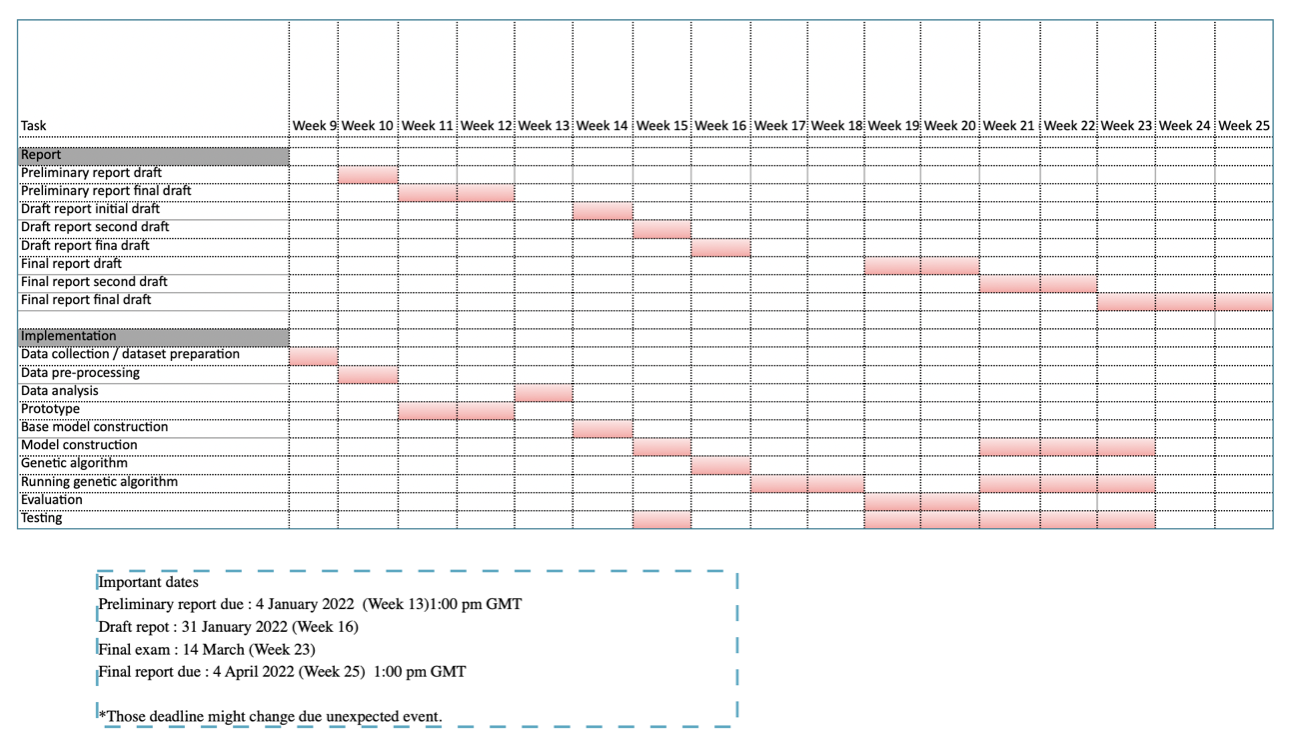
\includegraphics[width=\linewidth]{./gantt.png}
  \end{subfigure}

  \begin{subfigure}[b]{1.0\linewidth}
  \centering
  \caption{BiLSTM model with Conv1D}
  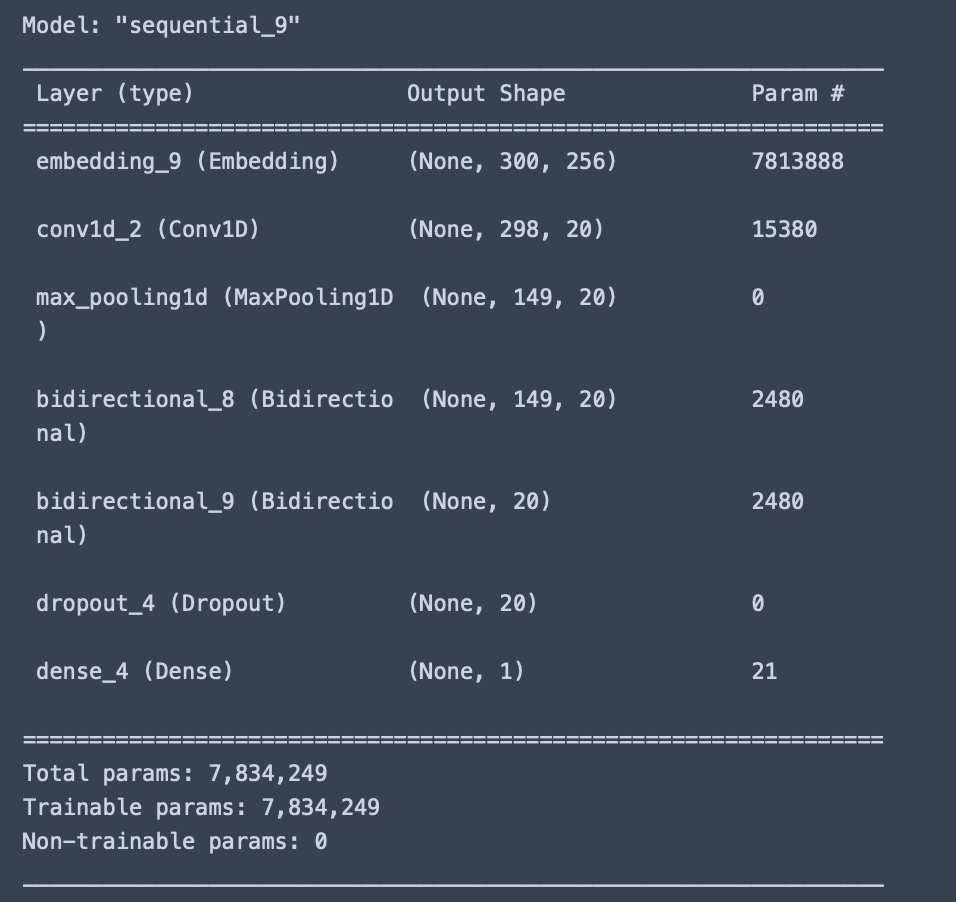
\includegraphics[width=0.5\textwidth]{./model.png}
  \end{subfigure}

  \begin{subfigure}[b]{1.0\linewidth}
  \centering
  \caption{Result of model prediction}
  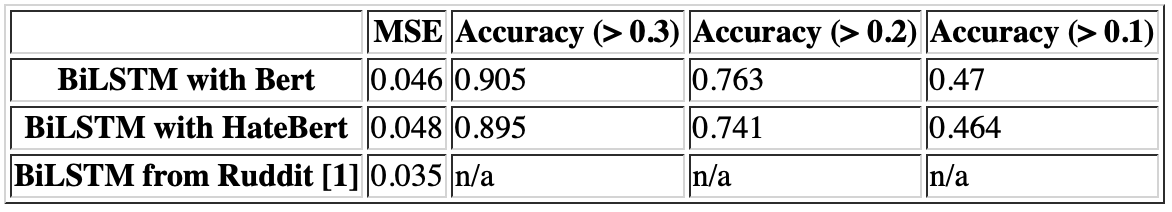
\includegraphics[width=0.5\textwidth]{./table1.png}
  \end{subfigure}

  \begin{subfigure}[b]{1.0\linewidth}
  \centering
  \caption{Code to convert comment ID to comment}
  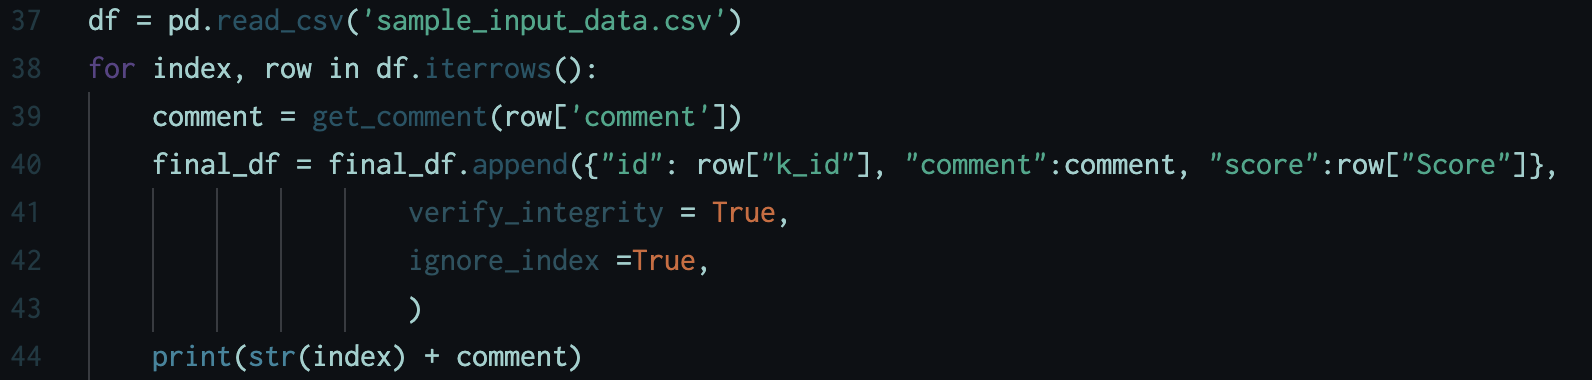
\includegraphics[width=0.5\textwidth]{./code.png}
  \end{subfigure}

\end{figure}
\end{document}
